\documentclass[11pt,a4paper]{report}
\usepackage[textwidth=37em,vmargin=30mm]{geometry}
\usepackage{calc,xunicode,amsmath,amssymb,paralist,enumitem,tabu,booktabs,datetime2,xeCJK,xeCJKfntef,listings}
\usepackage{tocloft,fancyhdr,tcolorbox,xcolor,graphicx,eso-pic,xltxtra,xelatexemoji}

\newcommand{\envyear}[0]{2025}
\newcommand{\envdatestr}[0]{2025-10-16}
\newcommand{\envfinaldir}[0]{webdb/2025/20251016/final}

\usepackage[hidelinks]{hyperref}
\hypersetup{
    colorlinks=false,
    pdfpagemode=FullScreen,
    pdftitle={Web Digest - \envdatestr}
}

\setlength{\cftbeforechapskip}{10pt}
\renewcommand{\cftchapfont}{\rmfamily\bfseries\large\raggedright}
\setlength{\cftbeforesecskip}{2pt}
\renewcommand{\cftsecfont}{\sffamily\small\raggedright}

\setdefaultleftmargin{2em}{2em}{1em}{1em}{1em}{1em}

\usepackage{xeCJK,xeCJKfntef}
\xeCJKsetup{PunctStyle=plain,RubberPunctSkip=false,CJKglue=\strut\hskip 0pt plus 0.1em minus 0.05em,CJKecglue=\strut\hskip 0.22em plus 0.2em}
\XeTeXlinebreaklocale "zh"
\XeTeXlinebreakskip = 0pt


\setmainfont{Brygada 1918}
\setromanfont{Brygada 1918}
\setsansfont{IBM Plex Sans}
\setmonofont{JetBrains Mono NL}
\setCJKmainfont{Noto Serif CJK SC}
\setCJKromanfont{Noto Serif CJK SC}
\setCJKsansfont{Noto Sans CJK SC}
\setCJKmonofont{Noto Sans CJK SC}

\setlength{\parindent}{0pt}
\setlength{\parskip}{8pt}
\linespread{1.15}

\lstset{
	basicstyle=\ttfamily\footnotesize,
	numbersep=5pt,
	backgroundcolor=\color{black!5},
	showspaces=false,
	showstringspaces=false,
	showtabs=false,
	tabsize=2,
	captionpos=b,
	breaklines=true,
	breakatwhitespace=true,
	breakautoindent=true,
	linewidth=\textwidth
}






\newcommand{\coverpic}[2]{
    % argv: itemurl, authorname
    Cover photo by #2~~(\href{#1}{#1})
}
\newcommand{\makeheader}[0]{
    \begin{titlepage}
        % \newgeometry{hmargin=15mm,tmargin=21mm,bmargin=12mm}
        \begin{center}
            
            \rmfamily\scshape
            \fontspec{BaskervilleF}
            \fontspec{Old Standard}
            \fontsize{59pt}{70pt}\selectfont
            WEB\hfill DIGEST
            
            \vfill
            % \vskip 30pt
            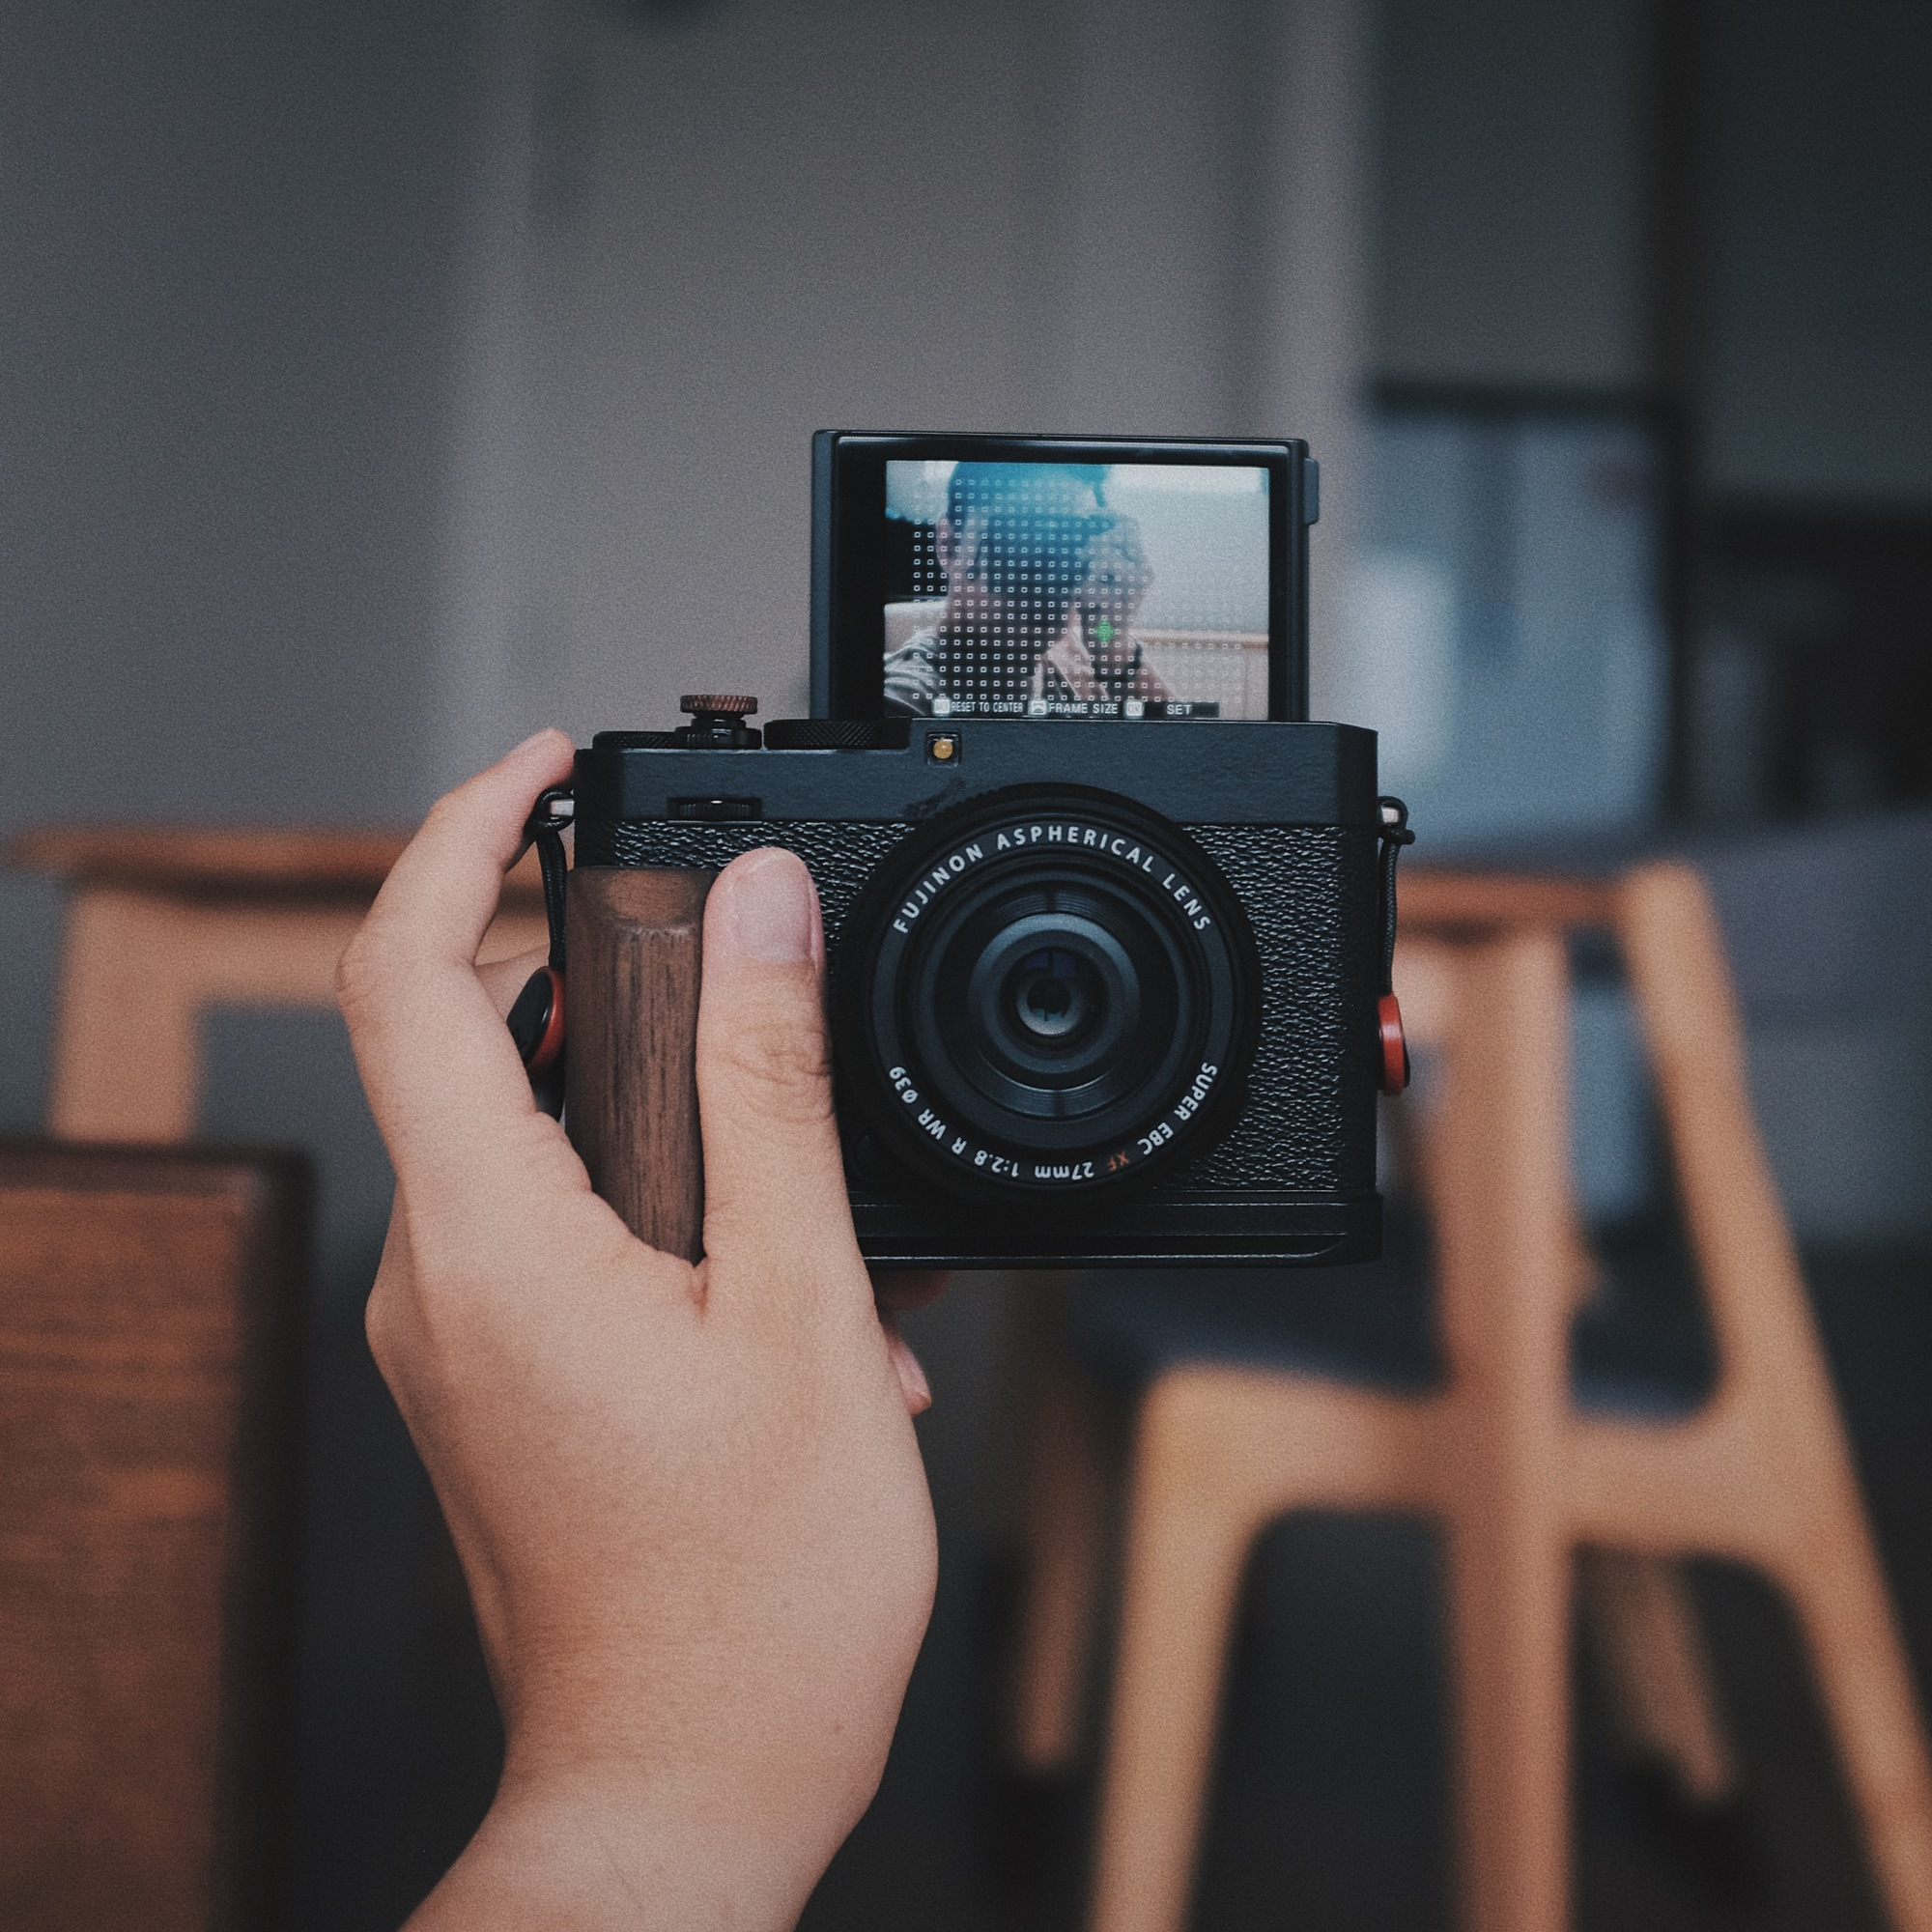
\includegraphics[width=\linewidth]{\envfinaldir/coverpic-prod.jpg}\par
            % \vskip 30pt
            \vfill

            \normalsize\rmfamily\scshape
            \copyright{} The Web Digest Project \hfill\large \envdatestr
        \end{center}
    \end{titlepage}
    % \restoregeometry
}
\newcommand{\simplehref}[1]{%
    \textcolor{blue!80!green}{\href{#1}{#1}}%
}
\renewcommand{\contentsname}{\center\Huge\sffamily\bfseries Contents\par\vskip 20pt}
\newcounter{ipartcounter}
\setcounter{ipartcounter}{0}
\newcommand{\ipart}[1]{
    % \vskip 20pt
    \clearpage
    \stepcounter{ipartcounter}
    \phantomsection
    \addcontentsline{toc}{chapter}{#1}
    % \begin{center}
    %     \Huge
    %     \sffamily\bfseries
    %     #1
    % \end{center}
    % \vskip 20pt plus 7pt
}
\newcounter{ichaptercounter}
\setcounter{ichaptercounter}{0}
\newcommand{\ichapter}[1]{
    % \vskip 20pt
    \clearpage
    \stepcounter{ichaptercounter}
    \phantomsection
    \addcontentsline{toc}{section}{\numberline{\arabic{ichaptercounter}}#1}
    \begin{center}
        \Huge
        \sffamily\bfseries
        #1
    \end{center}
    \vskip 20pt plus 7pt
}
\newcommand{\entrytitlefont}[1]{\subsection*{\raggedright\Large\sffamily\bfseries#1}}
\newcommand{\entryitemGeneric}[2]{
    % argv: title, url
    \parbox{\linewidth}{
        \entrytitlefont{#1}\par\vskip 5pt
        \footnotesize\ttfamily\mdseries
        \simplehref{#2}
    }\vskip 11pt plus 11pt minus 1pt
}
\newcommand{\entryitemGithub}[3]{
    % argv: title, url, desc
    \parbox{\linewidth}{
        \entrytitlefont{#1}\par\vskip 5pt
        \footnotesize\ttfamily\mdseries
        \simplehref{#2}\par\vskip 5pt
        \small\rmfamily\mdseries#3
    }\vskip 11pt plus 11pt minus 1pt
}
\newcommand{\entryitemAp}[3]{
    % argv: title, url, desc
    \parbox{\linewidth}{
        \entrytitlefont{#1}\par\vskip 5pt
        \footnotesize\ttfamily\mdseries
        \simplehref{#2}\par\vskip 5pt
        \small\rmfamily\mdseries#3
    }\vskip 11pt plus 11pt minus 1pt
}
\newcommand{\entryitemHackernews}[3]{
    % argv: title, hnurl, rawurl
    % \parbox{\linewidth}{
    %     \entrytitlefont{#1}\par\vskip 5pt
    %     \footnotesize\ttfamily\mdseries
    %     \simplehref{#3}\par
    %     \textcolor{black!50}{\href{#2}{#2}}
    % }\vskip 11pt plus 11pt minus 1pt
    \begin{minipage}{\linewidth}
            \entrytitlefont{#1}\par\vskip 5pt
            \footnotesize\ttfamily\mdseries
            \simplehref{#3}\par
            \textcolor{black!50}{\href{#2}{#2}}
    \end{minipage}\par\vskip 11pt plus 11pt minus 1pt
}







\begin{document}

\makeheader

\tableofcontents\clearpage




\ipart{Developers}
\ichapter{Hacker News}
\entryitemTwoLinks{I Hate Acrobat}{https://news.ycombinator.com/item?id=45598776}{https://www.vincentuden.xyz/blog/pdf-reader}

\entryitemTwoLinks{Getting syntax highlighting wrong}{https://news.ycombinator.com/item?id=45596960}{https://tonsky.me/blog/syntax-highlighting/}

\entryitemTwoLinks{Things I've learned in my 7 years implementing AI}{https://news.ycombinator.com/item?id=45596602}{https://www.jampa.dev/p/llms-and-the-lessons-we-still-havent}

\entryitemTwoLinks{US Passport Power Falls to Historic Low}{https://news.ycombinator.com/item?id=45595746}{https://www.henleyglobal.com/newsroom/press-releases/henley-global-mobility-report-oct-2025}

\entryitemTwoLinks{Are hard drives getting better?}{https://news.ycombinator.com/item?id=45595724}{https://www.backblaze.com/blog/are-hard-drives-getting-better-lets-revisit-the-bathtub-curve/}

\entryitemTwoLinks{Claude Haiku 4.5}{https://news.ycombinator.com/item?id=45595403}{https://www.anthropic.com/news/claude-haiku-4-5}

\entryitemTwoLinks{Zed is now available on Windows}{https://news.ycombinator.com/item?id=45594920}{https://zed.dev/blog/zed-for-windows-is-here}

\entryitemTwoLinks{You are the scariest monster in the woods}{https://news.ycombinator.com/item?id=45592766}{https://jamie.ideasasylum.com/2025/10/15/you-are-the-scariest-monster-in-the-woods}

\entryitemTwoLinks{A kernel stack use-after-free: Exploiting Nvidia's GPU Linux drivers}{https://news.ycombinator.com/item?id=45592585}{https://blog.quarkslab.com/./nvidia\_gpu\_kernel\_vmalloc\_exploit.html}

\entryitemTwoLinks{Pwning the Nix ecosystem}{https://news.ycombinator.com/item?id=45592401}{https://ptrpa.ws/nixpkgs-actions-abuse}

\entryitemTwoLinks{F5 says hackers stole undisclosed BIG-IP flaws, source code}{https://news.ycombinator.com/item?id=45592271}{https://www.bleepingcomputer.com/news/security/f5-says-hackers-stole-undisclosed-big-ip-flaws-source-code/}

\entryitemTwoLinks{iPad Pro with M5 chip}{https://news.ycombinator.com/item?id=45591905}{https://www.apple.com/newsroom/2025/10/apple-introduces-the-powerful-new-ipad-pro-with-the-m5-chip/}

\entryitemTwoLinks{M5 MacBook Pro}{https://news.ycombinator.com/item?id=45591902}{https://www.apple.com/macbook-pro/}

\entryitemTwoLinks{Mac Source Ports – Run old games on new Macs}{https://news.ycombinator.com/item?id=45591865}{https://www.macsourceports.com/}

\entryitemTwoLinks{Apple Vision Pro upgraded with M5 chip}{https://news.ycombinator.com/item?id=45591801}{https://www.apple.com/newsroom/2025/10/apple-vision-pro-upgraded-with-the-m5-chip-and-dual-knit-band/}

\entryitemTwoLinks{Apple M5 chip}{https://news.ycombinator.com/item?id=45591799}{https://www.apple.com/newsroom/2025/10/apple-unleashes-m5-the-next-big-leap-in-ai-performance-for-apple-silicon/}

\entryitemTwoLinks{I almost got hacked by a 'job interview'}{https://news.ycombinator.com/item?id=45591707}{https://blog.daviddodda.com/how-i-almost-got-hacked-by-a-job-interview}

\entryitemTwoLinks{Show HN: Scriber Pro – Offline AI transcription for macOS}{https://news.ycombinator.com/item?id=45591222}{https://scriberpro.cc/hn/}

\entryitemTwoLinks{Garbage collection for Rust: The finalizer frontier}{https://news.ycombinator.com/item?id=45591149}{https://soft-dev.org/pubs/html/hughes\_tratt\_\_garbage\_collection\_for\_rust\_the\_finalizer\_frontier/}

\entryitemTwoLinks{Show HN: Halloy – Modern IRC client}{https://news.ycombinator.com/item?id=45590949}{https://github.com/squidowl/halloy}\ichapter{Phoronix}
\entryitemGeneric{\hskip 0pt{}Valve Developer Contributes Open-Source Driver Fixes For 12 Year Old Hawaii GPUs}{https://www.phoronix.com/news/Valve-Fixes-2025-Hawaii-GPUs}

\entryitemGeneric{\hskip 0pt{}PyTorch 2.9 Released With Easier Install Support For AMD ROCm \& Intel XPUs}{https://www.phoronix.com/news/PyTorch-2.9-Released}

\entryitemGeneric{\hskip 0pt{}Mesa 25.2.5 Released With Very Important Intel Driver Fix}{https://www.phoronix.com/news/Mesa-25.2.5-Released}

\entryitemGeneric{\hskip 0pt{}Open 3D Engine O3DE 25.10 Brings Build Improvements, Vulkan \& Linux Fixes}{https://www.phoronix.com/news/Open-3D-O3DE-25.10}

\entryitemGeneric{\hskip 0pt{}Intel ISH Firmware Upstreamed Ahead Of Intel Panther Lake Laptops}{https://www.phoronix.com/news/Intel-ISH-Firmware-Panther-Lake}

\entryitemGeneric{\hskip 0pt{}AMD EPYC 9005 Brings Incredible Performance To The Cloud With Amazon M8a Benchmarks}{https://www.phoronix.com/review/ec2-m8a-amd-epyc-turin}

\entryitemGeneric{\hskip 0pt{}Apple Announces M5 With Much Faster GPU For AI}{https://www.phoronix.com/news/Apple-M5}

\entryitemGeneric{\hskip 0pt{}Tinygrad Gains A Mesa NIR Backend - Initially Supporting NVK/NAK \& LLVMpipe Execution}{https://www.phoronix.com/news/Tinygrad-Mesa-NIR-Backend}

\entryitemGeneric{\hskip 0pt{}AMD HIP-RT Is Stable For Blender 5.0 But Will Be Off By Default Until Blender 5.1}{https://www.phoronix.com/news/AMD-HIP-RT-Blender-5-Status}


\ipart{Developers~~~~(zh-Hans)}
\ichapter{Solidot}
\entryitemGeneric{\hskip 0pt{}研究发现卫星未加密传输敏感信息}{https://www.solidot.org/story?sid=82550}

\entryitemGeneric{\hskip 0pt{}商务部首次以 WPS 文档格式发表公告}{https://www.solidot.org/story?sid=82549}

\entryitemGeneric{\hskip 0pt{}女性被系统性的刻画成比男性更年轻}{https://www.solidot.org/story?sid=82548}

\entryitemGeneric{\hskip 0pt{}Google 限制 Android 侧载是其至今采取的最反消费者举措}{https://www.solidot.org/story?sid=82547}

\entryitemGeneric{\hskip 0pt{}NASA JPL 裁员 550 人}{https://www.solidot.org/story?sid=82546}

\entryitemGeneric{\hskip 0pt{}软件更新导致部分吉普牧马人 4xe 变砖}{https://www.solidot.org/story?sid=82545}

\entryitemGeneric{\hskip 0pt{}x86 生态系统顾问团队过去一年的成果}{https://www.solidot.org/story?sid=82544}

\entryitemGeneric{\hskip 0pt{}美国 AI 淘金热下制造业疲软}{https://www.solidot.org/story?sid=82543}

\entryitemGeneric{\hskip 0pt{}日本夏季过去 42 年增加了 3 周}{https://www.solidot.org/story?sid=82542}

\entryitemGeneric{\hskip 0pt{}教宗督促警惕控制算法的人}{https://www.solidot.org/story?sid=82541}

\entryitemGeneric{\hskip 0pt{}大部分开放权重模型都来自中国}{https://www.solidot.org/story?sid=82540}

\entryitemGeneric{\hskip 0pt{}微软终止对 windows 10 的支持}{https://www.solidot.org/story?sid=82539}

\entryitemGeneric{\hskip 0pt{}诺贝尔经济学奖授予了研究创新对经济影响的三名经济学家}{https://www.solidot.org/story?sid=82538}

\entryitemGeneric{\hskip 0pt{}SmartNav 将城市 GPS 精度提升到 10 厘米}{https://www.solidot.org/story?sid=82537}

\entryitemGeneric{\hskip 0pt{}高龄父亲会将更多致病突变遗传给后代}{https://www.solidot.org/story?sid=82536}

\entryitemGeneric{\hskip 0pt{}法拉利宣布首款电动跑车}{https://www.solidot.org/story?sid=82535}

\entryitemGeneric{\hskip 0pt{}Firefox 改进配置文件管理 }{https://www.solidot.org/story?sid=82534}

\entryitemGeneric{\hskip 0pt{}新生儿血液中的超级细菌十分普遍}{https://www.solidot.org/story?sid=82533}

\entryitemGeneric{\hskip 0pt{}流浪天体被发现可能是一颗反复爆发的亚恒星}{https://www.solidot.org/story?sid=82532}

\entryitemGeneric{\hskip 0pt{}金星大气层含水量超预期}{https://www.solidot.org/story?sid=82531}\ichapter{V2EX}
\entryitemGeneric{\hskip 0pt{}[Fluentd] 祝您今日愉快}{https://www.v2ex.com/t/1165968}

\entryitemGeneric{\hskip 0pt{}[问与答] 想买 iPhone17,有什么优惠渠道吗}{https://www.v2ex.com/t/1165967}

\entryitemGeneric{\hskip 0pt{}[程序员] 现在哪款显示器可 "仅关闭显示/背光"}{https://www.v2ex.com/t/1165966}

\entryitemGeneric{\hskip 0pt{}[分享发现] 做了一个免费的 AI 视频生成工具(用闲置 GPU 搭的)}{https://www.v2ex.com/t/1165965}

\entryitemGeneric{\hskip 0pt{}[Faucet] 还有机会领打赏吗?谢谢老板}{https://www.v2ex.com/t/1165964}

\entryitemGeneric{\hskip 0pt{}[搜索引擎优化] 创建了一个``论坛''}{https://www.v2ex.com/t/1165961}

\entryitemGeneric{\hskip 0pt{}[Faucet] 试一试能不能收到打赏}{https://www.v2ex.com/t/1165960}

\entryitemGeneric{\hskip 0pt{}[全球工单系统] @Cursor 这个 checkbox 是不是忘记画框了 bro?}{https://www.v2ex.com/t/1165958}

\entryitemGeneric{\hskip 0pt{}[加密货币] 购买 CMBMINT 后,币安 web3 为什么交易完后钱包里没有收到 CMBMINT 呢?}{https://www.v2ex.com/t/1165957}

\entryitemGeneric{\hskip 0pt{}[Faucet] 求第一个处女空投~}{https://www.v2ex.com/t/1165956}

\entryitemGeneric{\hskip 0pt{}[Faucet] 大佬你看我还有机会吗}{https://www.v2ex.com/t/1165955}

\entryitemGeneric{\hskip 0pt{}[MacBook Pro] 下单了 M5 MacBook Pro 32+512}{https://www.v2ex.com/t/1165954}

\entryitemGeneric{\hskip 0pt{}[Faucet] 求空投~}{https://www.v2ex.com/t/1165953}

\entryitemGeneric{\hskip 0pt{}[电动汽车] 请问下家冲桩的蓝牙要是坏了一般在哪里换啊}{https://www.v2ex.com/t/1165952}

\entryitemGeneric{\hskip 0pt{}[OpenAI] 跟 openAI 学日语,选的是女声,这个是女声吗?}{https://www.v2ex.com/t/1165951}

\entryitemGeneric{\hskip 0pt{}[程序员] 作为后端程序员在 cursor 加持下写前端,最适合的前端框架/方案?}{https://www.v2ex.com/t/1165949}

\entryitemGeneric{\hskip 0pt{}[程序员] 大家一般开发的场景下使用多少个屏幕,一般怎么摆放?}{https://www.v2ex.com/t/1165948}

\entryitemGeneric{\hskip 0pt{}[宠物] 发现程序员 it 男普遍喜欢养猫 不喜欢养狗}{https://www.v2ex.com/t/1165947}

\entryitemGeneric{\hskip 0pt{}[Windows] Windows Update 疑难杂症}{https://www.v2ex.com/t/1165945}

\entryitemGeneric{\hskip 0pt{}[机械键盘] 大家的机械键盘是什么轴?}{https://www.v2ex.com/t/1165944}

\entryitemGeneric{\hskip 0pt{}[问与答] 一加 13 回锁失败变砖}{https://www.v2ex.com/t/1165943}

\entryitemGeneric{\hskip 0pt{}[Faucet] 让我看看怎么回事儿}{https://www.v2ex.com/t/1165941}

\entryitemGeneric{\hskip 0pt{}[Faucet] 新人贴 来凑个热闹🔥}{https://www.v2ex.com/t/1165940}

\entryitemGeneric{\hskip 0pt{}[iPad] 2025 年你还会购买 iPad 吗 主要用来做啥?}{https://www.v2ex.com/t/1165938}

\entryitemGeneric{\hskip 0pt{}[Android] 安卓 TV 开机启动类似轮播的视频播放应用?}{https://www.v2ex.com/t/1165937}

\entryitemGeneric{\hskip 0pt{}[Faucet] 等大佬的空投,谢谢大佬!}{https://www.v2ex.com/t/1165936}

\entryitemGeneric{\hskip 0pt{}[Faucet] 来财来 来空投}{https://www.v2ex.com/t/1165935}

\entryitemGeneric{\hskip 0pt{}[Faucet] 听说发帖能得到打赏,我也来试试}{https://www.v2ex.com/t/1165934}

\entryitemGeneric{\hskip 0pt{}[问与答] 后端小组成员怎么分层}{https://www.v2ex.com/t/1165933}

\entryitemGeneric{\hskip 0pt{}[Faucet] 我想看看这些赛博要饭贴最后怎么收场}{https://www.v2ex.com/t/1165932}

\entryitemGeneric{\hskip 0pt{}[Faucet] 支持支持,赞赞赞}{https://www.v2ex.com/t/1165931}

\entryitemGeneric{\hskip 0pt{}[Faucet] 这就不得不发一个了}{https://www.v2ex.com/t/1165930}

\entryitemGeneric{\hskip 0pt{}[Faucet] 等一个空投,老板大气!}{https://www.v2ex.com/t/1165929}

\entryitemGeneric{\hskip 0pt{}[Faucet] faucet 不就是 solana 空投吗?我也来领空投。}{https://www.v2ex.com/t/1165927}

\entryitemGeneric{\hskip 0pt{}[分享发现] 为什么感觉 Grok 在回答一般性问题(非代码)上还不错}{https://www.v2ex.com/t/1165926}

\entryitemGeneric{\hskip 0pt{}[分享创造] 做的一个 Discord Decoration web 应用,玩 discord 的,过来瞧瞧,欢迎拍砖}{https://www.v2ex.com/t/1165925}

\entryitemGeneric{\hskip 0pt{}[iOS] 求教几个 LLDB 技巧/逆向技巧}{https://www.v2ex.com/t/1165922}

\entryitemGeneric{\hskip 0pt{}[Faucet] 1111,真有空投?}{https://www.v2ex.com/t/1165920}

\entryitemGeneric{\hskip 0pt{}[MacBook Pro] MacBook Pro M5 芯片来了}{https://www.v2ex.com/t/1165919}

\entryitemGeneric{\hskip 0pt{}[Faucet] 老板大气,恭喜发财}{https://www.v2ex.com/t/1165918}

\entryitemGeneric{\hskip 0pt{}[酷工作] 深圳|前端求职}{https://www.v2ex.com/t/1165916}

\entryitemGeneric{\hskip 0pt{}[iPad] 电信和移动这次开放 esim 之后 iPad pro 可以用吗}{https://www.v2ex.com/t/1165915}

\entryitemGeneric{\hskip 0pt{}[Faucet] 跟风体验一下,刚创建了一个账号}{https://www.v2ex.com/t/1165914}

\entryitemGeneric{\hskip 0pt{}[职场话题] 你们对于要求应聘者开摄像头,自己却不开的情况怎么看?}{https://www.v2ex.com/t/1165913}

\entryitemGeneric{\hskip 0pt{}[Faucet] 要到饭了兄弟们!}{https://www.v2ex.com/t/1165912}

\entryitemGeneric{\hskip 0pt{}[Faucet] 谢主打赏}{https://www.v2ex.com/t/1165911}

\entryitemGeneric{\hskip 0pt{}[Faucet] 一个合格的测试号}{https://www.v2ex.com/t/1165910}

\entryitemGeneric{\hskip 0pt{}[Node.js] [EvanNav 6.3.1] 如何删除加载页面,让 Nav 更符合你的需求⁉️}{https://www.v2ex.com/t/1165908}

\entryitemGeneric{\hskip 0pt{}[分享发现] 地主家也没有余粮了 [EdgeOne] 关于免费套餐下线源站防护功能的通知}{https://www.v2ex.com/t/1165907}

\entryitemGeneric{\hskip 0pt{}[求职] 重庆 Java /.NET 程序员重庆求职}{https://www.v2ex.com/t/1165906}


\ipart{Generic News}







\clearpage
\leavevmode\vfill
\footnotesize

Copyright \copyright{} 2023-2025 Neruthes and other contributors.

This document is published with CC BY-NC-ND 4.0 license.

The entries listed in this newsletter may be copyrighted by their respective creators.

This newsletter is generated by the Web Digest project.

The newsletters are also delivered via Telegram channel \CJKunderline{\href{https://t.me/webdigestchannel}{https://t.me/webdigestchannel}}.\\
RSS feed is available at \CJKunderline{\href{https://webdigest.pages.dev/rss.xml}{https://webdigest.pages.dev/rss.xml}}.

This newsletter is available in PDF at
\CJKunderline{\href{https://webdigest.pages.dev/}{https://webdigest.pages.dev/}}.

The source code being used to generate this newsletter is available at\\
\CJKunderline{\href{https://github.com/neruthes/webdigest}{https://github.com/neruthes/webdigest}}.

This newsletter is also available in
\CJKunderline{\href{http://webdigest.pages.dev/readhtml/\envyear/WebDigest-20251016.html}{HTML}} and
\CJKunderline{\href{https://github.com/neruthes/webdigest/blob/master/markdown/\envyear/WebDigest-20251016.md}{Markdown}}.


\coverpic{https://unsplash.com/photos/pink-flowers-are-in-full-bloom-against-the-blue-sky-ZKcUj8la0aY}{HLS 44}


\end{document}
